% ------------------------------------------------------------------------------
% TYPO3 CMS 8.0 - What's New (English Version)
%
% @author	Patrick Lobacher <patrick@lobacher.de> and Michael Schams <schams.net>
% @license	Creative Commons BY-NC-SA 3.0
% @link		http://typo3.org/download/release-notes/whats-new/
% @language	English
% ------------------------------------------------------------------------------
% LTXE-CHAPTER-UID:		d71b4b88-f79b2343-d2b356bf-452cef81
% LTXE-CHAPTER-NAME:	Backend User Interface
% ------------------------------------------------------------------------------

\section{Interfaccia utente Backend}
\begin{frame}[fragile]
	\frametitle{Interfaccia utente Backend}

	\begin{center}\huge{Capitolo 1:}\end{center}
	\begin{center}\huge{\color{typo3darkgrey}\textbf{Interfaccia utente Backend}}\end{center}

\end{frame}

% ------------------------------------------------------------------------------
% LTXE-SLIDE-START
% LTXE-SLIDE-UID:		833531e7-3501c939-2972e779-6130a38e
% LTXE-SLIDE-ORIGIN:	d8599a04-11b4fa8c-9be5812a-715820e1 English
% LTXE-SLIDE-ORIGIN:	ef1d6d8c-0db67396-dedb5814-1767169f German
% LTXE-SLIDE-TITLE:		Recover pages recursively to top of rootline
% LTXE-SLIDE-REFERENCE:	!Feature-1835-RecoverPagesRecursivelyToTop.rst
% ------------------------------------------------------------------------------
\begin{frame}[fragile]
	\frametitle{Interfaccia utente Backend}
	\framesubtitle{Recupero ricorsivo delle pagine dalla rootline}

	Il cestino supporta il ripristino ricorsivo delle pagine cancellate dalla rootline.
	Questa funzionalità è disponibile solo per gli utenti amministratori per delle restrizioni di permessi interne.

	\begin{figure}
		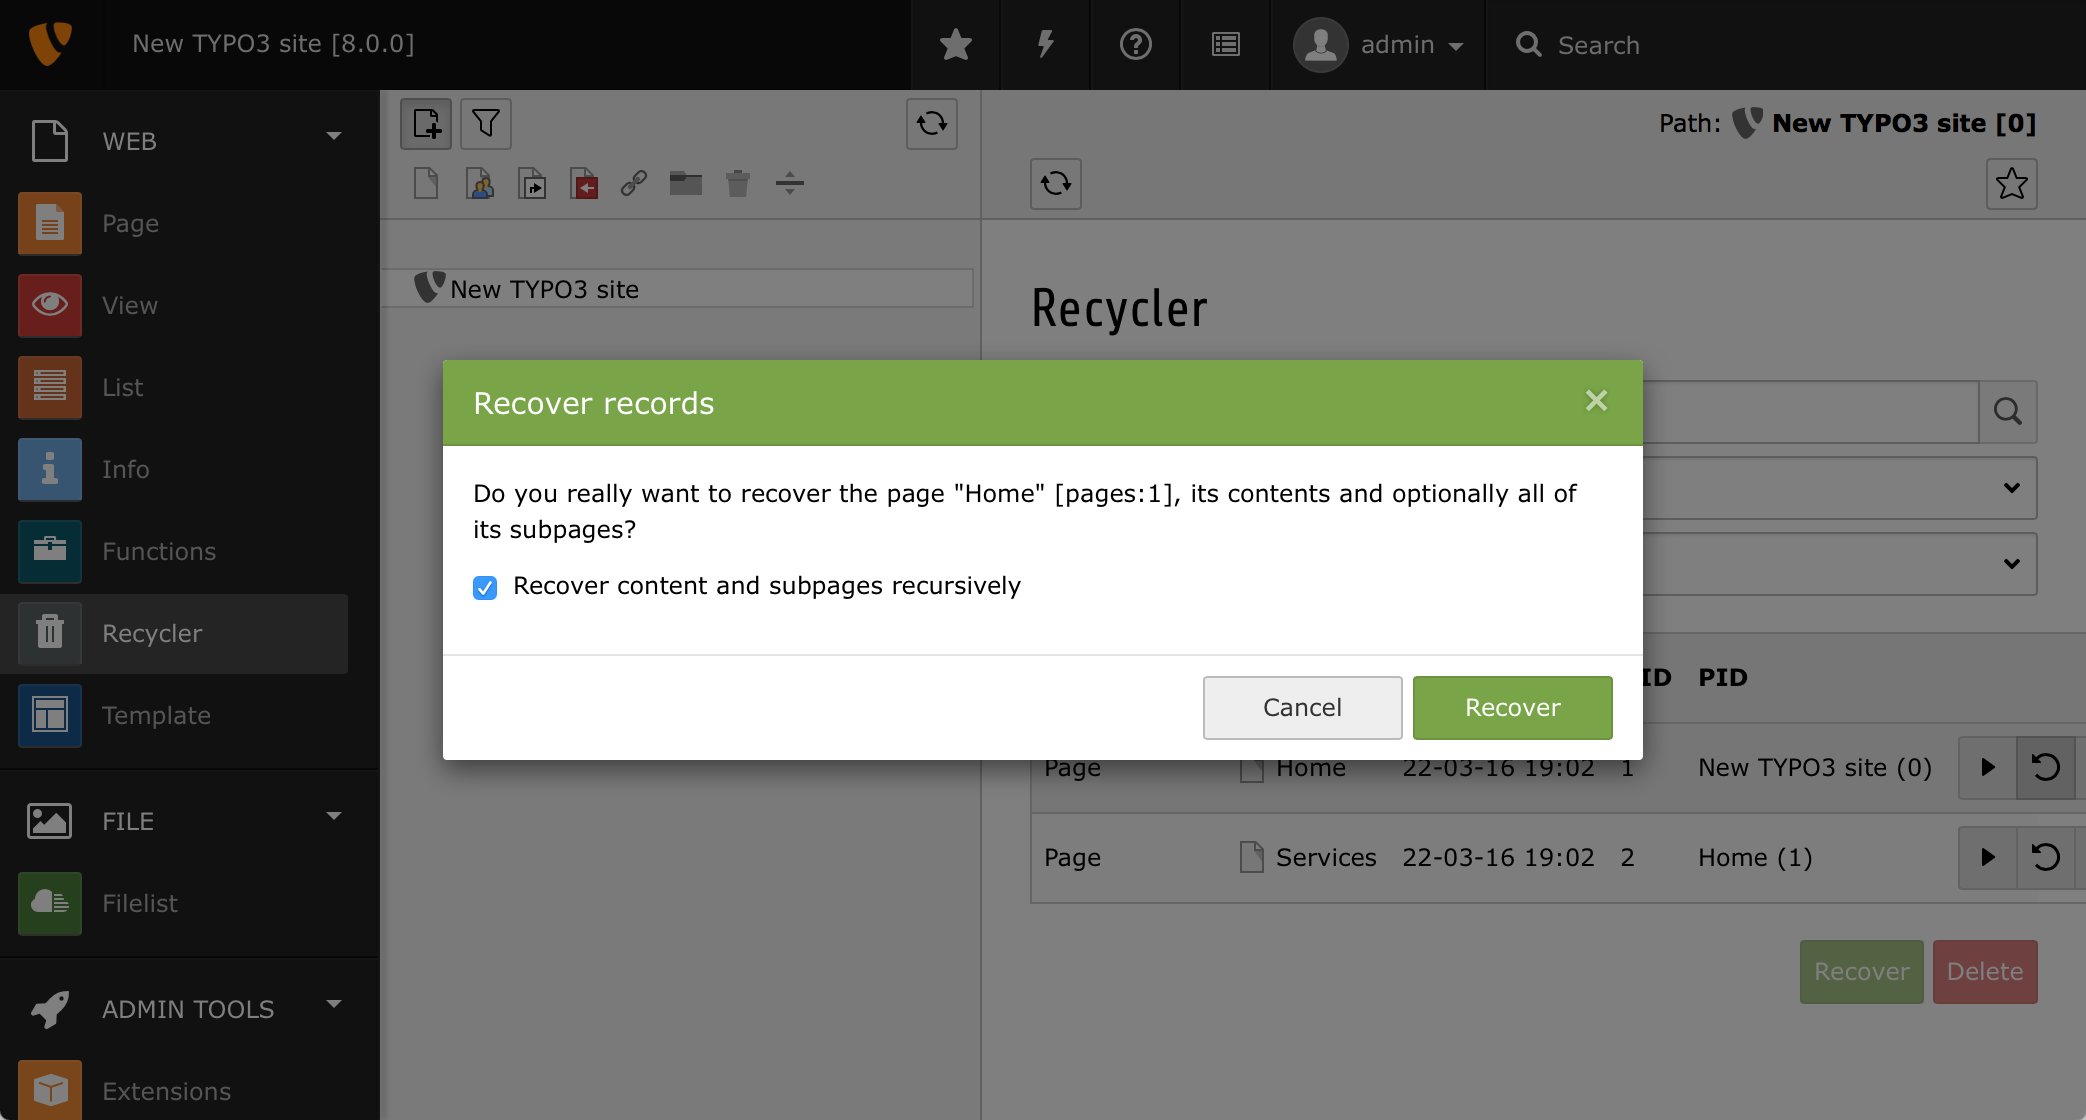
\includegraphics[width=0.70\linewidth]{BackendUserInterface/1835.png}
	\end{figure}

\end{frame}

% ------------------------------------------------------------------------------
% LTXE-SLIDE-START
% LTXE-SLIDE-UID:		784dd319-fc9f308b-aebacaa7-1f2485bf
% LTXE-SLIDE-ORIGIN:	04855567-dac16e24-f5274c64-f1d49c36 English
% LTXE-SLIDE-TITLE:		EXT:form - Directly load form wizard as inline wizard
% LTXE-SLIDE-REFERENCE:	!Feature-69394-EXTform-DirectlyLoadFormWizardAsInlineWizard.rst
% ------------------------------------------------------------------------------
\begin{frame}[fragile]
	\frametitle{Interfaccia utente Backend}
	\framesubtitle{Caricamento diretto del wizard dei form come wizard in linea}

	Il wizard dell'EXT:form è caricato direttamente come wizard in linea.
	Non è più necessario salvare e ricaricare un nuovo elemento di contenuto con
	lo scopo di poter aprire il wizard. Si tratta di un enorme miglioramento di usabilità.

	\begin{figure}
		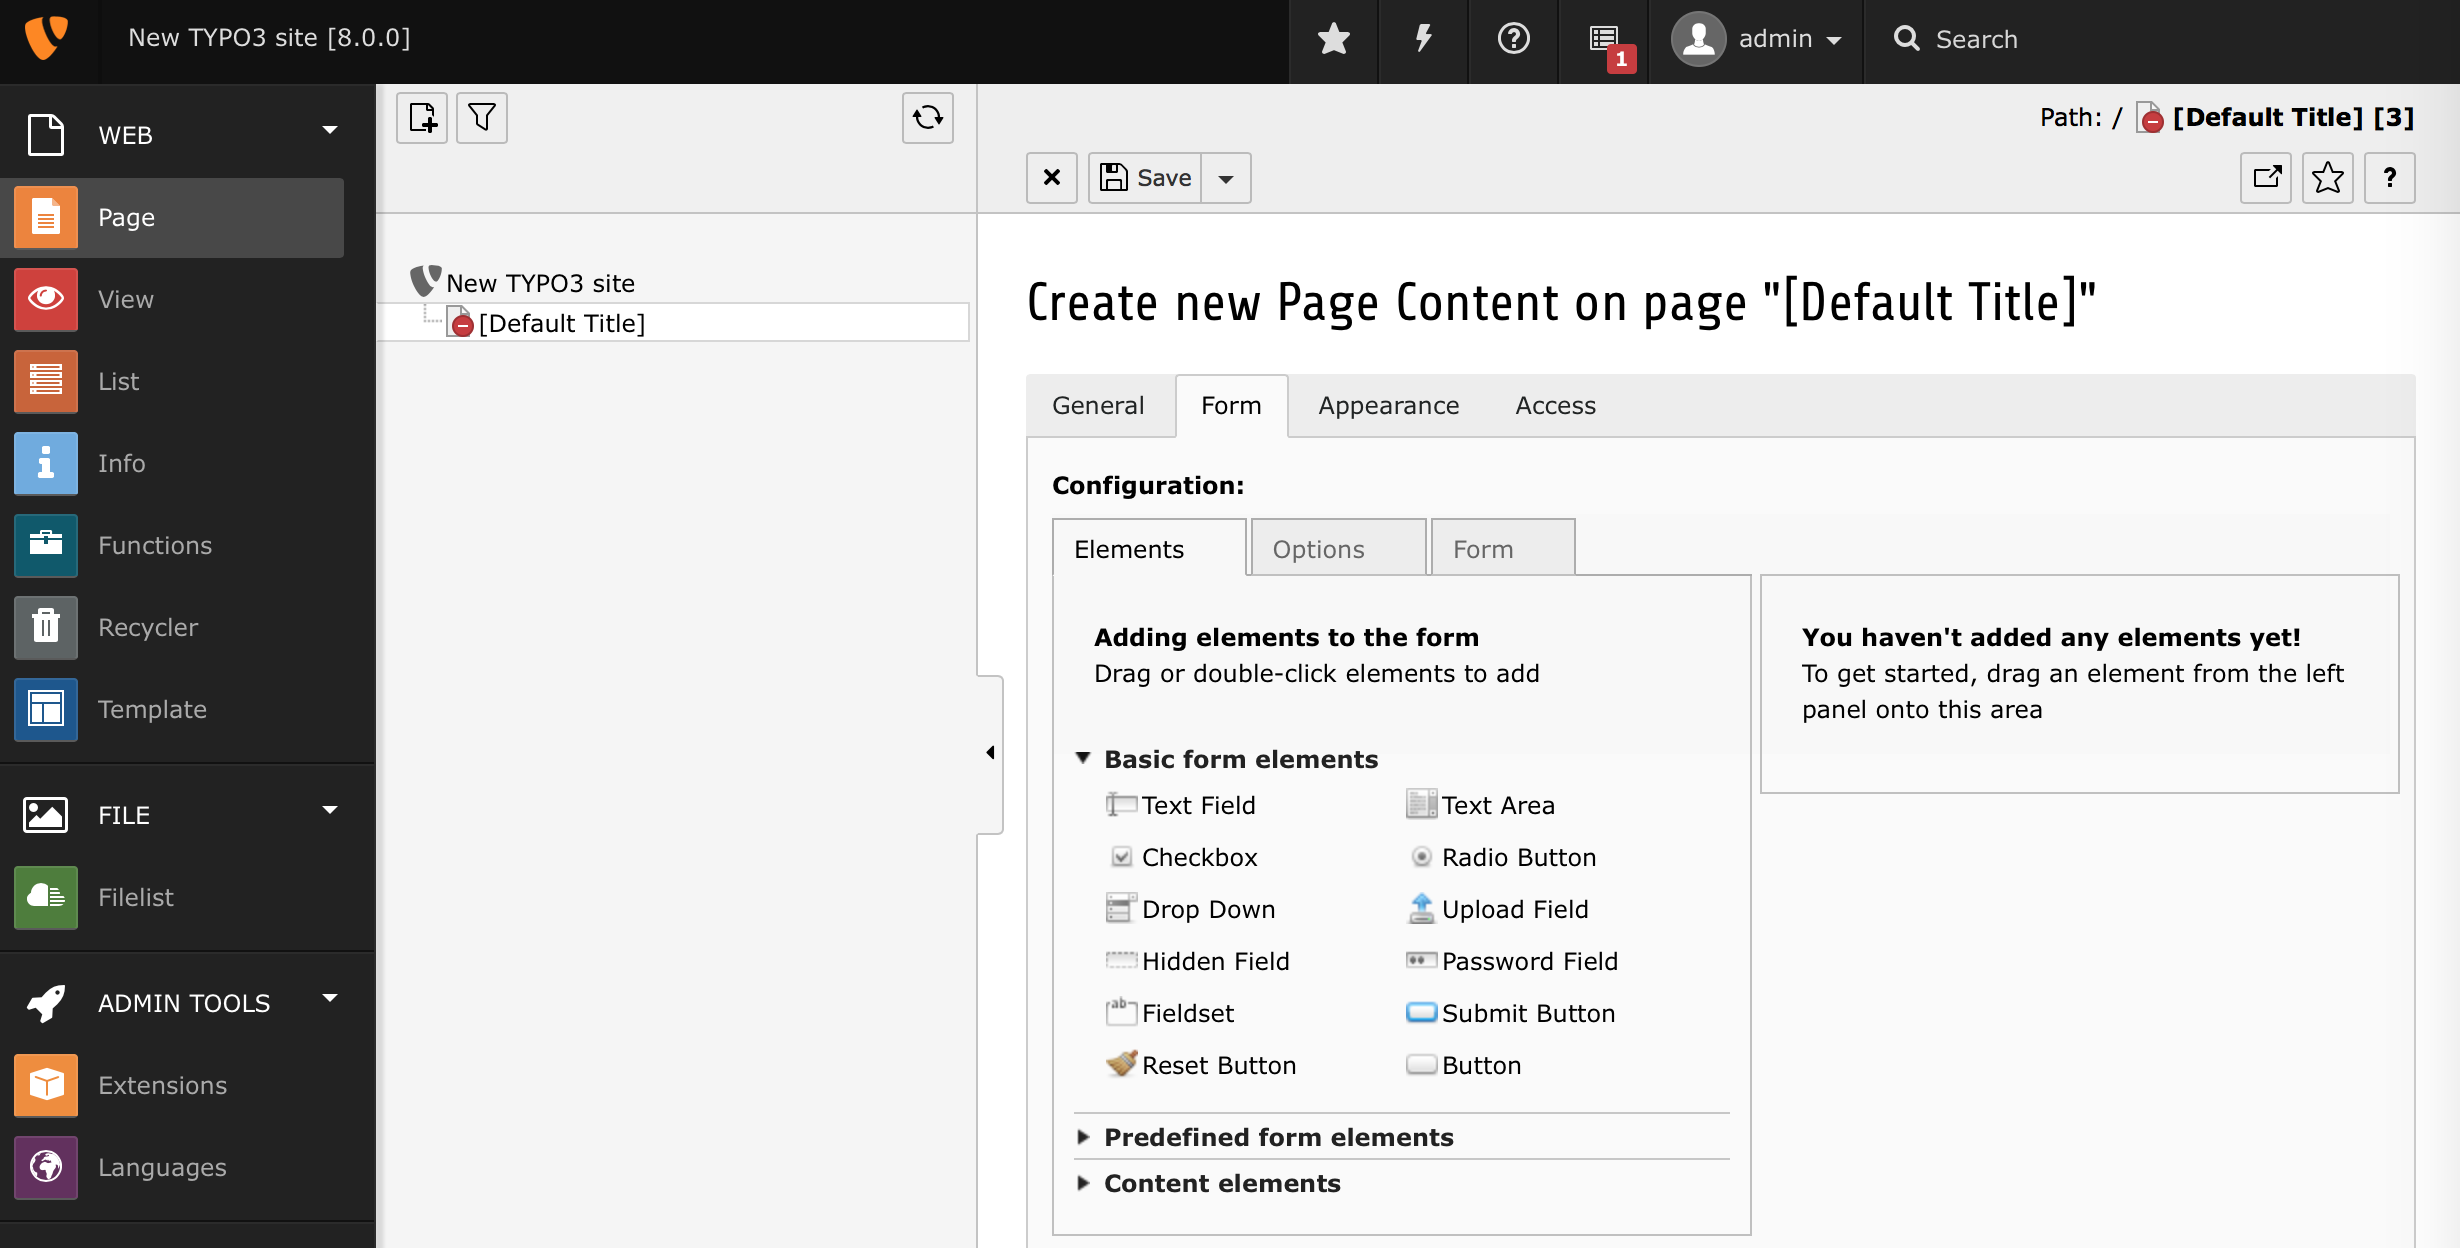
\includegraphics[width=0.70\linewidth]{BackendUserInterface/69394.png}
	\end{figure}

\end{frame}

% ------------------------------------------------------------------------------
% LTXE-SLIDE-START
% LTXE-SLIDE-UID:		fd4d56a4-995bae09-24d6735b-9e297f8e
% LTXE-SLIDE-ORIGIN:	fd6d762a-b268caf0-cb6f9195-f553e035 English
% LTXE-SLIDE-TITLE:		Set the alternative backend logo via Extension Manager
% LTXE-SLIDE-REFERENCE:	!Feature-74109-SetTheAlternativeBackendLogoViaExtensionManager.rst
% ------------------------------------------------------------------------------
\begin{frame}[fragile]
	\frametitle{Interfaccia utente Backend}
	\framesubtitle{Impostare un logo di backend alternativo via Extension Manager}

	Il logo di backend, nell'angolo in alto a sinistra, può ora essere configurato nelle configurazioni
	dell'estensione EXT:backend nell'Extension Manager.\newline
	Le opzioni di configurazione sono:

	\begin{itemize}
		\item risorsa come percorso relativo dell'installazione TYPO3\newline
			\smaller
				es. "\texttt{fileadmin/images/my-background.jpg}"
			\normalsize

		\item percorso ad un estensione\newline
			\smaller
				es. "\texttt{EXT:my\_theme/Resources/Public/Images/my-background.jpg}"
			\normalsize

		\item una risorsa esterna\newline
			\smaller
				es. "\texttt{//example.com/my-background.png}"
			\normalsize

	\end{itemize}

	\begin{figure}
		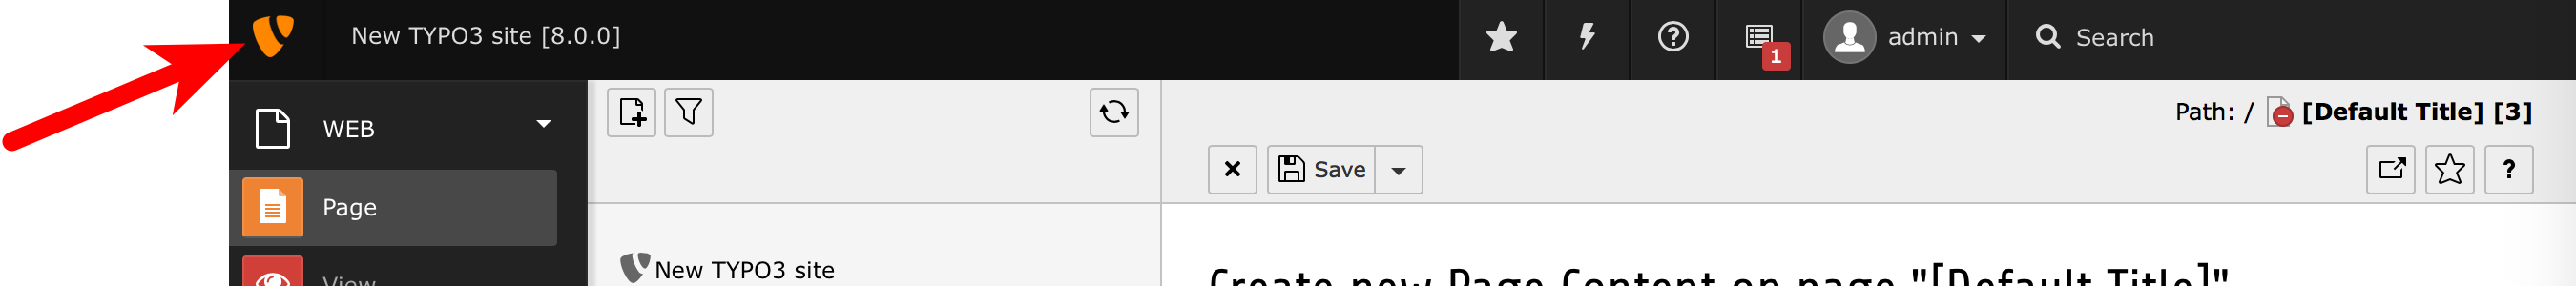
\includegraphics[width=0.7\linewidth]{BackendUserInterface/74109.png}
	\end{figure}

\end{frame}

% ------------------------------------------------------------------------------
% LTXE-SLIDE-START
% LTXE-SLIDE-UID:		fad3deeb-b499e321-ff3dea34-8f7ee49a
% LTXE-SLIDE-ORIGIN:	ab5ef36b-c670fbea-fd6d762a-cb6f9195 English
% LTXE-SLIDE-TITLE:		Page module: drag and drop supports copying now
% LTXE-SLIDE-REFERENCE:	!Feature-74179-PageModuleDragDropCanDoCopiesViaCTRLKeyNow.rst
% ------------------------------------------------------------------------------
\begin{frame}[fragile]
	\frametitle{Interfaccia utente Backend}
	\framesubtitle{Copia delle pagine in modalità drag \& drop}

	In aggiunta alla tradizionale funzionalità drag and drop nel modulo della pagina (che \textit{muove} gli elementi di contenuto),
	è ora possibile creare delle copie: premere il tasto CTRL mentre si trascina un elemento per copiarlo.
	Dopo che il rilascio è completato, il modulo della pagina viene ricaricato per esser sicuri che il nuovo elemento
	sia stato generato con tutte le informazioni necessarie.

	\begin{figure}
		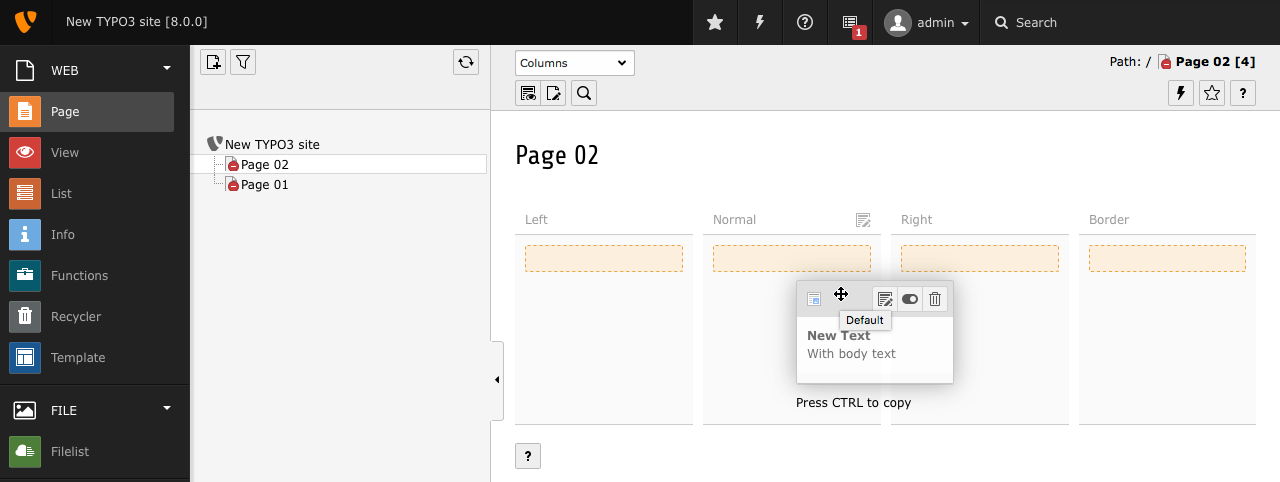
\includegraphics[width=0.7\linewidth]{BackendUserInterface/74179.png}
	\end{figure}

\end{frame}

% ------------------------------------------------------------------------------
